%picture
\documentclass{article}
\usepackage{graphicx}
\usepackage{subfigure}
\usepackage{epstopdf}
\graphicspath{{figures/}}%说明图片位置
\begin{document}
picture feild

    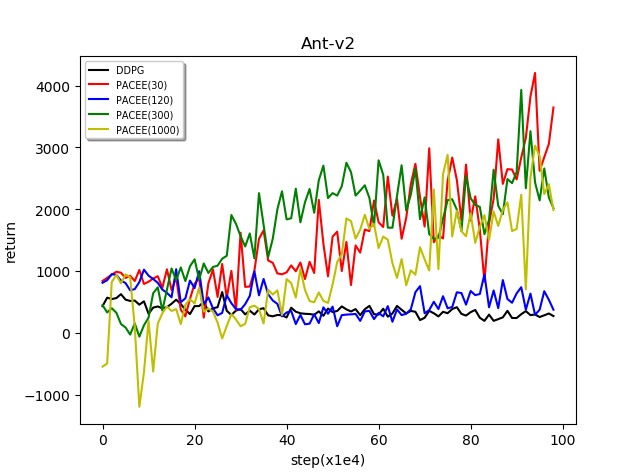
\includegraphics{Ant}
    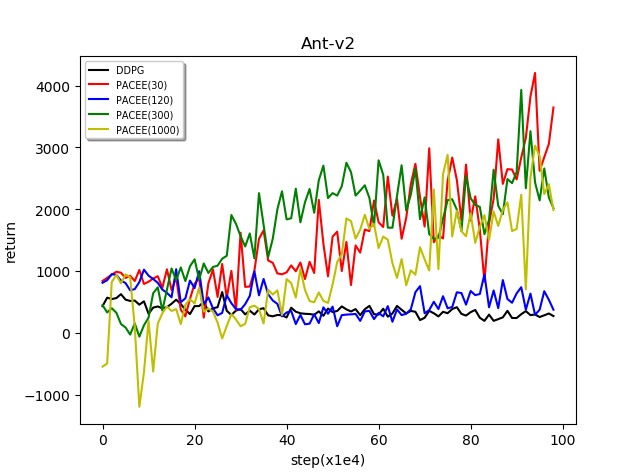
\includegraphics[height=3cm]{Ant}
    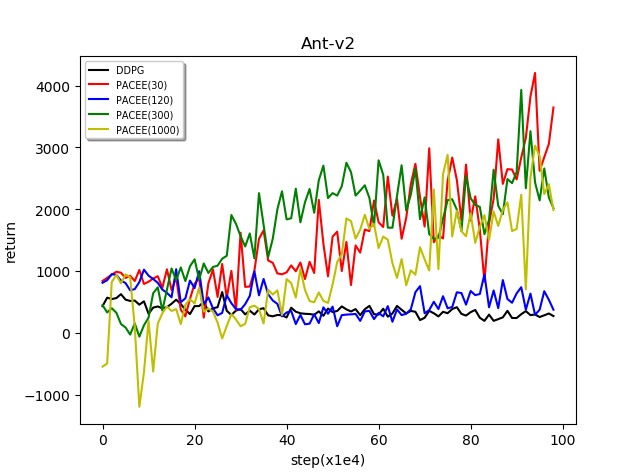
\includegraphics[width=4cm]{Ant}

    the next picture is \ref{Ant2}

    \begin{figure}[htbp]
      \centering
      \includegraphics[width=5cm]{ant}
      \caption{Ant,average on 10 trials}\label{Ant}
      \includegraphics[width=5cm]{ant}
      \caption{ant,average on 10 trial}\label{Ant2}%每个subfigure之间不能有空格
    \end{figure}
    \begin{figure}[h]
        \centering
        \subfigure[pic1.]{
        \begin{minipage}[t]{0.25\linewidth}
        \centering
        \includegraphics[width=1in]{ant}
        %\caption{fig1}
        \end{minipage}%
        }%
        \subfigure[pic2.]{
        \begin{minipage}[t]{0.25\linewidth}
        \centering
        \includegraphics[width=1in]{ant}
        %\caption{fig2}
        \end{minipage}%
        }%
        \subfigure[pic3.]{
        \begin{minipage}[t]{0.25\linewidth}%这里指每张图片之间距离是0.25倍行宽
        \centering
        \includegraphics[width=1in]{ant}
        %\caption{fig2}
        \end{minipage}
        }%
        \subfigure[pic4.]{
        \begin{minipage}[t]{0.25\linewidth}
        \centering
        \includegraphics[width=1in]{ant}
        %\caption{fig2}
        \end{minipage}
        }%
        \centering
        \caption{ pics}
    \end{figure}
    second figure:

    \begin{figure}[h]
      \centering

      \subfigure[ant]{
        \begin{minipage}[t]{0.25\linewidth}
          \centering
          \includegraphics[width=3cm]{ant}
        \end{minipage}
      }
      \subfigure[hopper]{
        \begin{minipage}[t]{0.25\linewidth}
          \centering
          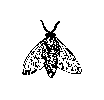
\includegraphics[width=3cm]{fly}
        \end{minipage}
              }

      \subfigure[hopper]{
        \begin{minipage}[t]{0.25\linewidth}
          \centering
          \includegraphics[width=3cm]{hopper}
        \end{minipage}
              }
      \subfigure[hopper]{
        \begin{minipage}[t]{0.25\linewidth}
          \centering
          \includegraphics[width=3cm]{hopper}
        \end{minipage}
              }

      \centering
      \caption{simulation result}\label{simulation}
    \end{figure}

    third subfigure,  second figure:  second figure:  second figure:  second figure:  second figure:  second figure:  second figure:  second figure:  second figure:  second figure:  second figure:  second figure:  second figure:  second figure:  second figure:  second figure:  second figure:  second figure:  second figure:  second figure:  second figure:  second figure:  second figure:  second figure:  second figure:  second figure:  second figure:  second figure:  second figure:  second figure:  second figure:  second figure:  second figure:  second figure:  second figure:

    \begin{figure}[h]
        \centering
        \subfigure[pic1.]{
        \begin{minipage}[t]{0.25\linewidth}
        \centering
        \includegraphics[width=1in]{ant}
        %\caption{fig1}
        \end{minipage}%
        }%
        \subfigure[pic2.]{
        \begin{minipage}[t]{0.25\linewidth}
        \centering
        \includegraphics[width=1in]{ant}
        %\caption{fig2}
        \end{minipage}%
        }%
                         %这个回车键很重要 \quad也可以
        \subfigure[pic3.]{
        \begin{minipage}[t]{0.25\linewidth}
        \centering
        \includegraphics[width=1in]{ant}
        %\caption{fig2}
        \end{minipage}
        }%
        \subfigure[pic4.]{
        \begin{minipage}[t]{0.25\linewidth}
        \centering
        \includegraphics[width=1in]{ant}
        %\caption{fig2}
        \end{minipage}
        }%
        \centering
        \caption{ pics}
   \end{figure}

\end{document} 